\section{测试、运行情况}

\subsection{测试情况}

本程序的每一个实验模块由组员完成后,组长会进行代码审核与测试,
如果发现问题则要求继续修改,直到所有问题被解决后该实验模块才会发布。
我们还建立了用户 QQ 群,并即时反馈用户提出的任何问题。

另一方面,各种 API 的编写与模块化编程也让我们的程序在编写过程中更不容易出错,
同时规范、统一的码风也让调试变得轻松。

\subsection{运行情况}

本项目从 2022 年 4 月 27 日上线以来,有超过 9000 次的浏览量,总访客数达到了 2100。

% \begin{figure}[htbp]
%   \centering
%   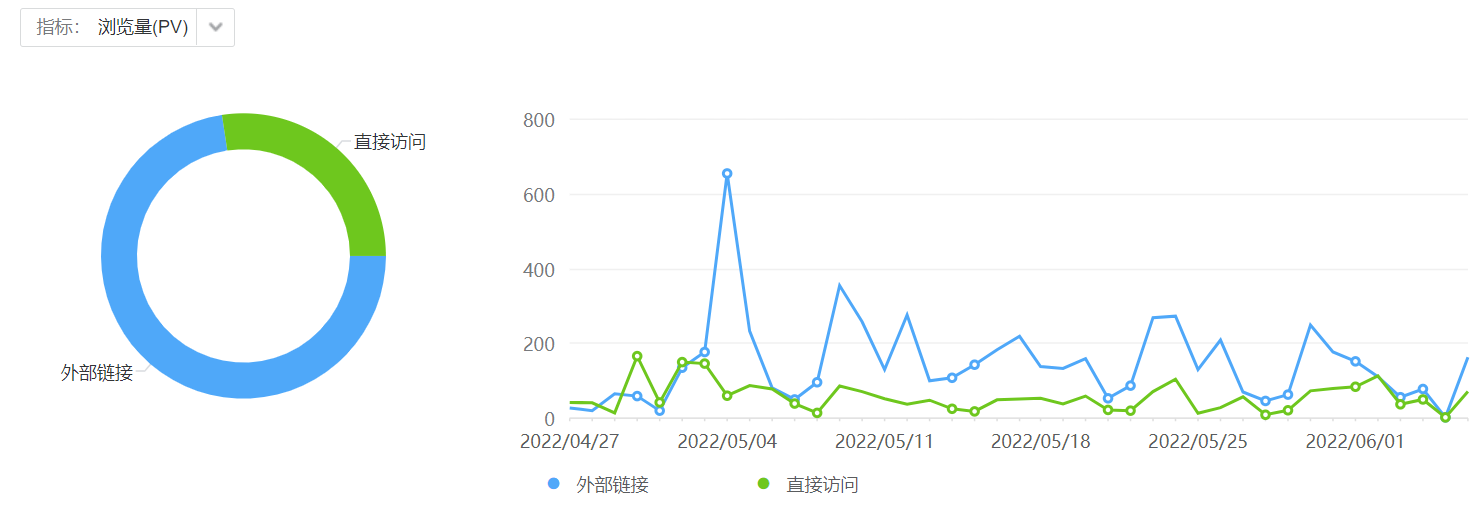
\includegraphics[width=\columnwidth]{figure/0.png}
%   \caption{4 月 27 日至 6 月 7 日的网站浏览量}
%   \label{fig:0}
% \end{figure}
% \begin{figure}[htbp]
%   \centering
%   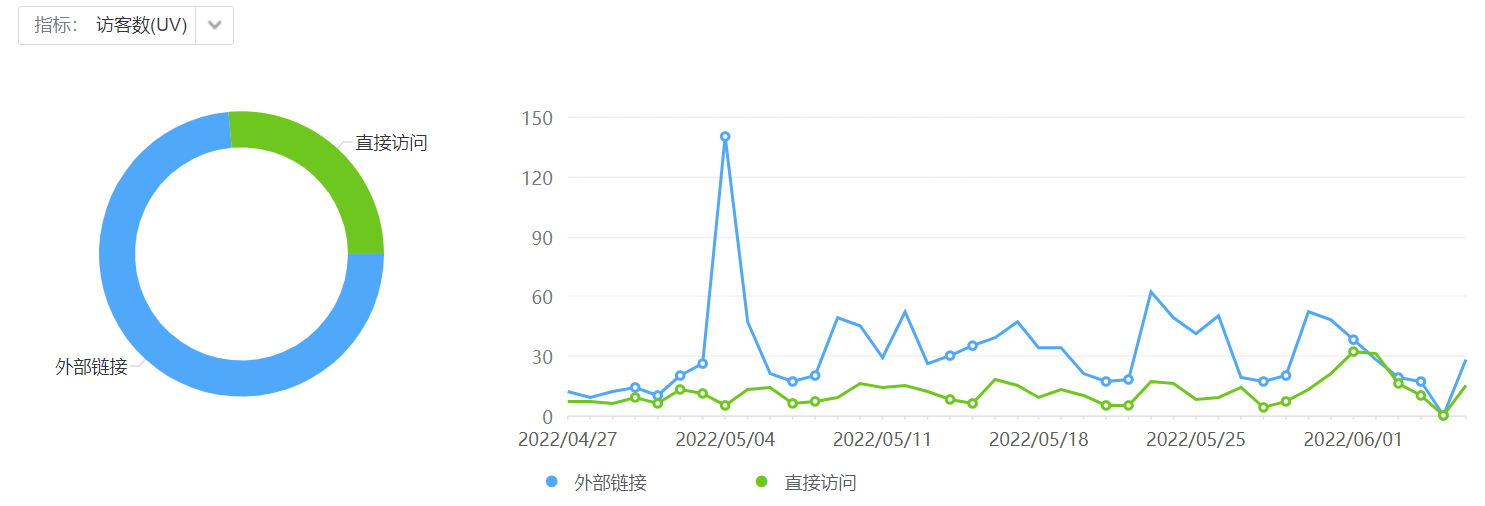
\includegraphics[width=\columnwidth]{figure/1.png}
%   \caption{4 月 27 日至 6 月 7 日的网站访客数}
%   \label{fig:1}
% \end{figure}

最后一次大物实验于 2022 年 6 月 3 日结束。
在大物实验结束之前,平均每天约有 50 名同学访问了我们网站,如图 \ref{fig:2} 所示。
考虑到每天只有不到 400 名大一学生做大物实验,本程序的使用率相对较高。
用户的平均访问时长为 6 分 36 秒,这说明我们的大雾实验工具非常简明易用。

\begin{figure}[htbp]
  \centering
  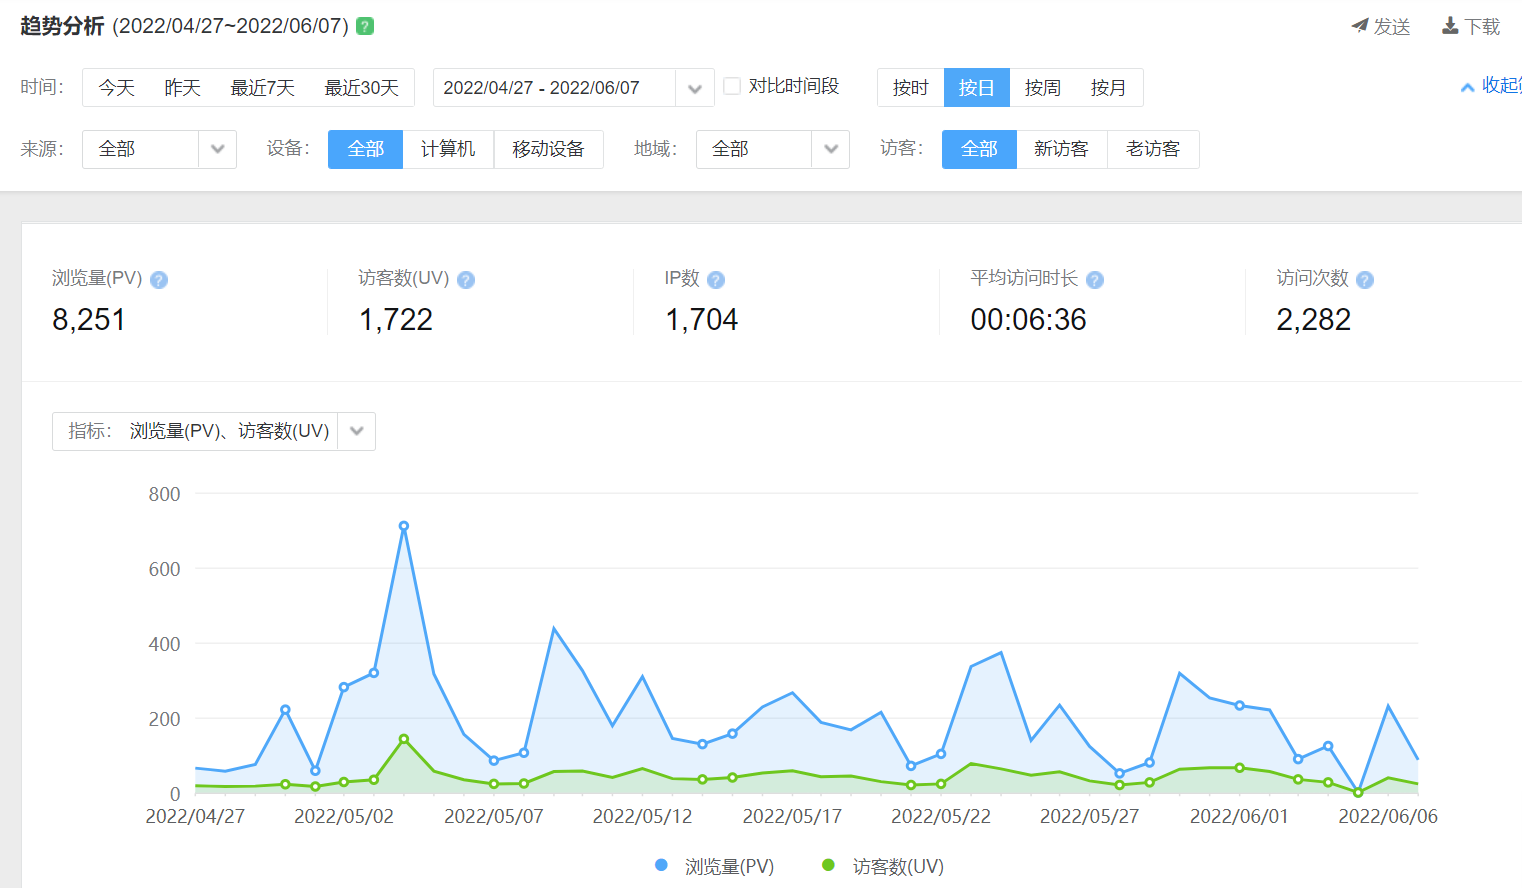
\includegraphics[width=\columnwidth]{figure/2.png}
  \caption{4 月 27 日至 6 月 6 日的统计数据}
  \label{fig:2}
\end{figure}